% Project report: Oak Hold'em (Java Programming).
% Build: tectonic -X compile report.tex   (or xelatex/pdflatex twice)
\documentclass[12pt,a4paper]{article}

\usepackage{iftex}
\ifXeTeX
  \usepackage{fontspec}
  \setmainfont{texgyretermes}[Extension=.otf, UprightFont=*-regular, BoldFont=*-bold,
    ItalicFont=*-italic, BoldItalicFont=*-bolditalic]
  \setsansfont{texgyreheros}[Extension=.otf, Scale=0.95, UprightFont=*-regular,
    BoldFont=*-bold, ItalicFont=*-italic, BoldItalicFont=*-bolditalic]
\else
  \usepackage[T1]{fontenc}
  \usepackage{newtxtext,newtxmath}
\fi
\usepackage[margin=2.5cm]{geometry}
\usepackage{graphicx}
\usepackage{booktabs}
\usepackage{array}
\usepackage{tabularx}
\usepackage{xcolor}
\usepackage{listings}
\usepackage{float}
\usepackage{caption}
\usepackage{subcaption}
\usepackage{tikz}
\usetikzlibrary{positioning,arrows.meta}
\usepackage{setspace}
\usepackage{fancyhdr}
\usepackage{etoolbox}
\usepackage{needspace}
% Keep each code listing on one page.
\BeforeBeginEnvironment{lstlisting}{\par\noindent\begin{minipage}{\linewidth}}
\AfterEndEnvironment{lstlisting}{\end{minipage}\par\medskip}
\usepackage[colorlinks=true,linkcolor=black,urlcolor=blue!60!black]{hyperref}

\onehalfspacing
\sloppy  % long class names in \texttt must not run into the margin
\captionsetup{font=small,labelfont=bf}
\newcolumntype{L}{>{\raggedright\arraybackslash}X}

\definecolor{codebg}{RGB}{247,247,244}
\definecolor{codekw}{RGB}{0,72,140}
\definecolor{codecm}{RGB}{110,110,110}
\definecolor{codestr}{RGB}{160,40,40}
\lstset{
  language=Java, basicstyle=\ttfamily\footnotesize, keywordstyle=\color{codekw}\bfseries,
  commentstyle=\color{codecm}\itshape, stringstyle=\color{codestr}, backgroundcolor=\color{codebg},
  frame=single, rulecolor=\color{black!15}, framesep=4pt, xleftmargin=6pt, xrightmargin=6pt,
  breaklines=true, columns=fullflexible, keepspaces=true, showstringspaces=false,
  numbers=left, numberstyle=\tiny\color{codecm}, numbersep=8pt, tabsize=4,
  morekeywords={record,var,sealed,permits}, aboveskip=8pt, belowskip=4pt,
  literate={’}{{'}}1
}
\renewcommand{\lstlistingname}{Code}

\pagestyle{fancy}
\fancyhf{}
\fancyhead[L]{\small Oak Hold'em: Project Report}
\fancyhead[R]{\small Java Programming}
\fancyfoot[C]{\small\thepage}
\renewcommand{\headrulewidth}{0.4pt}

\newcommand{\cls}[1]{\texttt{#1}}
\newcommand{\repo}{\url{https://github.com/SakD2006/holdem}}

\begin{document}

% ---------------------------------------------------------------- Cover
\begin{titlepage}
\centering
\vspace*{1.5cm}
{\large\textsc{Project Report}\par}
\vspace{1.2cm}
{\Huge\bfseries Oak Hold'em\par}
\vspace{0.4cm}
{\Large A multiplayer Texas Hold'em game for a local network, written in Java\par}
\vspace{0.3cm}
{\large (Poker Engine with AI Agents)\par}
\vspace{1.6cm}
{\large Course: \textbf{Java Programming}\par}
\vspace{0.3cm}
{\large Faculty: \textbf{Dr. Sharmila C}\par}
\vspace{1.6cm}
{\large\textbf{Submitted by}\par}
\vspace{0.4cm}
\begin{tabular}{ll}
\toprule
Name & Registration number \\
\midrule
Saksham Dubey & 24BBS0081 \\
Aryaman Sodha & 24BBS0110 \\
Tanay Doshi & 24BBS0104 \\
\bottomrule
\end{tabular}
\vfill
{\large Source code: \repo\par}
\vspace{0.6cm}
{\large October 2026\par}
\end{titlepage}

% ---------------------------------------------------------------- Abstract
\section*{Abstract}
\addcontentsline{toc}{section}{Abstract}

Oak Hold'em is a desktop poker game in which friends on the same local network (a home Wi-Fi or
a college lab) play No-Limit Texas Hold'em against each other and against computer players.
One computer runs the server and the database; every other player starts the desktop app, finds
the server, signs in, and either creates a room, which gives a six-character room code, or joins
one with a code. The room's creator starts the game.

The project is written in Java 21 as six Maven modules. A pure rules engine deals the cards,
runs the betting, splits side pots and ranks hands. A Tomcat server holds the rooms, talks to
the players over WebSockets, saves every hand to PostgreSQL through JDBC and to text files, and
serves a few JSP pages (leaderboard, room results, hand replays) to any browser on the network.
A JavaFX app is what people play on. Computer players come in three levels, the strongest of
which remembers how each opponent plays. The server never trusts the client and never sends a
player anyone else's cards.

The project uses every topic of the course syllabus: packages, abstract classes, inheritance,
polymorphism, user-defined exceptions, file handling, collections, JavaFX, JDBC, servlets, JSP
and multithreading. It contains about 19,500 lines of application code and more than 470
automated tests.

\newpage
{\singlespacing\tableofcontents}
\newpage

% ---------------------------------------------------------------- 1
\section{Introduction}

\subsection{The game}
Texas Hold'em is the most widely played form of poker. Each player is dealt two private cards
(\emph{hole cards}). Five shared cards (the \emph{board}) are then dealt face up in three
stages: three cards (the \emph{flop}), one (the \emph{turn}) and one more (the \emph{river}).
There is a round of betting before the flop and after each stage. In each round a player may
fold, check, call, bet or raise. In \emph{No-Limit} Hold'em a player may bet any amount up to
all their chips. A hand ends when everyone but one player has folded, or at the
\emph{showdown}, where the best five-card hand made from a player's two cards and the board wins
the pot. Hands rank, from strongest: straight flush, four of a kind, full house, flush, straight,
three of a kind, two pair, one pair, high card.

\subsection{Problem and aim}
Playing poker with friends usually needs either a physical deck and chips or an online site
that needs an internet account. The aim of this project is a small, self-contained program that
a group can run in one room on one network, with no internet and no installation beyond Java.

\subsection{Objectives}
\begin{itemize}
\item Play correct No-Limit Hold'em for 2 to 9 players, including all-ins and side pots.
\item Let players create and join rooms with a short code, with the creator as host.
\item Keep the game fair: the server checks every action and never reveals hidden cards.
\item Save accounts and every finished hand, and show a leaderboard and hand replays.
\item Offer computer players for when there are not enough people.
\item Use, visibly, each Java topic in the course syllabus.
\end{itemize}

% ---------------------------------------------------------------- 2
\section{System overview}

Figure~\ref{fig:arch} shows how the parts fit together. The \emph{host machine} runs the
server and PostgreSQL. Each player's computer runs the desktop app, which talks to the server
in two ways: plain HTTP requests carrying JSON for signing in and managing rooms, and a
WebSocket connection for the game itself, over which the server pushes every event the moment
it happens.

\begin{figure}[H]
\centering
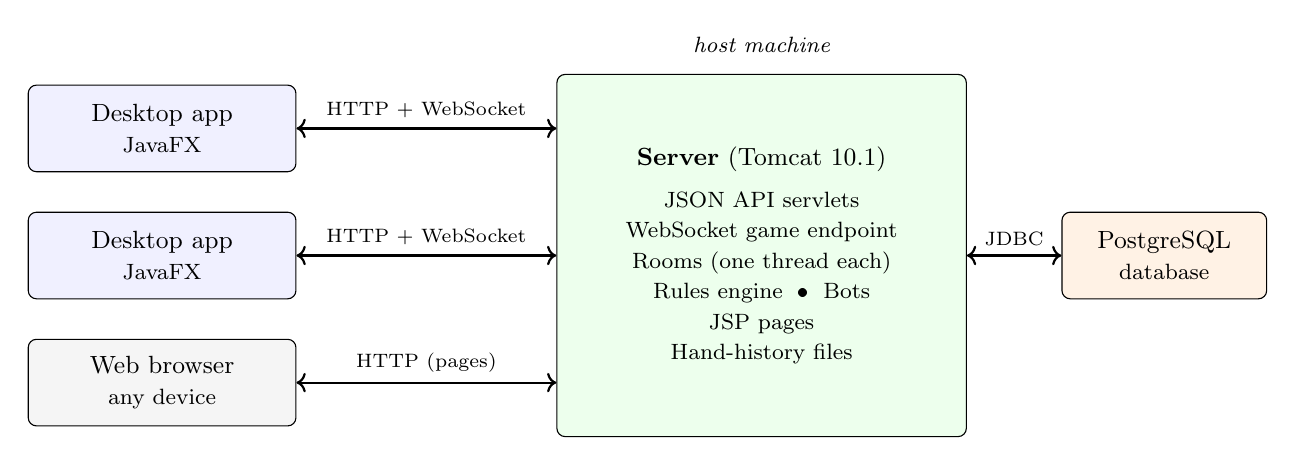
\begin{tikzpicture}[
  box/.style={draw, rounded corners=3pt, align=center, minimum height=1.1cm, inner sep=5pt,
              font=\small, fill=#1},
  box/.default=white,
  arr/.style={-{Stealth[length=2.2mm]}, thick}]
\node[box=blue!6, minimum width=3.4cm] (app1) {Desktop app\\\footnotesize JavaFX};
\node[box=blue!6, minimum width=3.4cm, below=0.5cm of app1] (app2) {Desktop app\\\footnotesize JavaFX};
\node[box=gray!8, minimum width=3.4cm, below=0.5cm of app2] (browser) {Web browser\\\footnotesize any device};
\node[box=green!7, minimum width=5.2cm, minimum height=4.6cm, right=3.3cm of app2, align=center] (server)
  {\textbf{Server} (Tomcat 10.1)\\[4pt]
   \footnotesize JSON API servlets\\ \footnotesize WebSocket game endpoint\\
   \footnotesize Rooms (one thread each)\\ \footnotesize Rules engine \;\textbullet\; Bots\\
   \footnotesize JSP pages\\ \footnotesize Hand-history files};
\node[box=orange!10, minimum width=2.6cm, right=1.2cm of server] (db) {PostgreSQL\\\footnotesize database};
\draw[arr, <->] (app1.east) -- node[above, font=\scriptsize] {HTTP + WebSocket} (server.west |- app1.east);
\draw[arr, <->] (app2.east) -- node[above, font=\scriptsize] {HTTP + WebSocket} (server.west);
\draw[arr, <->] (browser.east) -- node[above, font=\scriptsize] {HTTP (pages)} (server.west |- browser.east);
\draw[arr, <->] (server.east) -- node[above, font=\scriptsize] {JDBC} (db.west);
\node[font=\footnotesize\itshape, above=0.15cm of server] {host machine};
\end{tikzpicture}
\caption{Architecture. Every player connects to the one server on the local network.}
\label{fig:arch}
\end{figure}

Four rules shape the design:
\begin{enumerate}
\item \textbf{The server decides.} Clients only ask (``I raise to 600''); the server checks the
request against the rules before anything changes.
\item \textbf{Hidden cards stay hidden.} A player's hole cards are sent only to that player
until the showdown. This filtering happens in one class, \cls{EventRouter}.
\item \textbf{One thread per room.} Only a room's own thread changes that room, so the game
logic needs no locks.
\item \textbf{Bots see only what a person would.} A computer player receives exactly the
messages a person in its seat would receive.
\end{enumerate}

\begin{table}[H]
\centering\small
\caption{Technology used.}
\begin{tabularx}{\textwidth}{@{}lL@{}}
\toprule
Area & Technology \\
\midrule
Language and build & Java 21, Maven (multi-module, with the Maven wrapper) \\
Server & Apache Tomcat 10.1: Servlet 6, JSP 3.1 with JSTL 3, WebSocket 2.1 \\
Database & PostgreSQL 16, JDBC with the HikariCP connection pool \\
Desktop app & JavaFX 21; the JDK's \cls{java.net.http} client for HTTP and WebSocket \\
Data format & JSON through the Jackson library \\
Testing & JUnit 5 and AssertJ \\
Logging & SLF4J with Logback \\
\bottomrule
\end{tabularx}
\end{table}

% ---------------------------------------------------------------- 3
\section{Project modules}

The code is split into six Maven modules. Each one is a separate folder with its own
\cls{pom.xml} and produces its own JAR (the server produces a WAR). The arrows in
Figure~\ref{fig:modules} show which module uses which; nothing points the other way, so, for
example, the rules engine knows nothing about networks, databases or windows.

\begin{figure}[H]
\centering
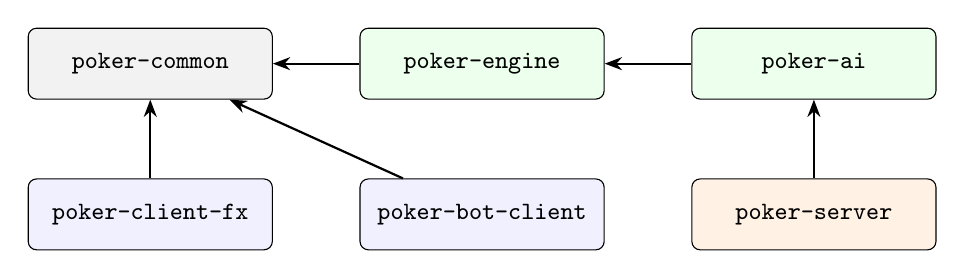
\begin{tikzpicture}[
  m/.style={draw, rounded corners=3pt, minimum width=3.1cm, minimum height=0.9cm, font=\small\ttfamily, fill=#1},
  m/.default=white,
  arr/.style={-{Stealth[length=2.2mm]}, thick}]
\node[m=gray!10] (common) {poker-common};
\node[m=green!7, right=1.1cm of common] (engine) {poker-engine};
\node[m=green!7, right=1.1cm of engine] (ai) {poker-ai};
\node[m=orange!10, below=1.0cm of ai] (server) {poker-server};
\node[m=blue!6, below=1.0cm of common] (client) {poker-client-fx};
\node[m=blue!6, below=1.0cm of engine] (bot) {poker-bot-client};
\draw[arr] (engine) -- (common);
\draw[arr] (ai) -- (engine);
\draw[arr] (server) -- (ai);
\draw[arr] (client) -- (common);
\draw[arr] (bot) -- (common);
\end{tikzpicture}
\caption{Module dependencies. An arrow means ``uses''.}
\label{fig:modules}
\end{figure}

\begin{table}[H]
\centering\small
\caption{Size of each module (main code only; tests are separate).}
\begin{tabular}{@{}lrrr@{}}
\toprule
Module & Java files & Lines & Test classes \\
\midrule
\cls{poker-common}     & 104 & 2,478 & 5 \\
\cls{poker-engine}     &  31 & 1,881 & 10 \\
\cls{poker-ai}         &  27 & 2,474 & 9 \\
\cls{poker-server}     &  74 & 6,182 & 26 \\
\cls{poker-client-fx}  &  43 & 5,725 & 12 \\
\cls{poker-bot-client} &   5 &   759 & 1 \\
\midrule
Total                  & 284 & 19,499 & 63 \\
\bottomrule
\end{tabular}
\end{table}

\subsection{poker-common: shared vocabulary}
\textbf{What it is.} The types that both the server and the clients need: cards, player
actions, every message sent over the network, error codes and the exception classes. It has no
input or output of its own.

\textbf{Main packages.} \cls{card} (\cls{Card}, \cls{Rank}, \cls{Suit}); \cls{action}
(the \cls{PlayerAction} hierarchy: fold, check, call, bet, raise, all-in); \cls{protocol}
(the abstract \cls{Message} class with about 40 client and server messages); \cls{exception}
(the \cls{PokerException} tree); \cls{lan} (the message format for finding a server on the
network).

\textbf{Usage.} Because the server and the app use the very same message classes, Jackson turns
a message into JSON on one side and back into the same Java object on the other.

\subsection{poker-engine: the rules of the game}
\textbf{What it is.} A pure implementation of No-Limit Hold'em. It deals, runs each betting
round, works out who may do what, builds the main pot and side pots, ranks hands and pays the
winners.

\textbf{Main packages.} \cls{card} (\cls{Deck}, \cls{DeckFactory}); \cls{hand} (\cls{Hand}, the
state machine for one hand, and \cls{BettingRound}); \cls{pot} (\cls{PotCalculator}); \cls{eval}
(\cls{HandEvaluator}, \cls{HandValue}); \cls{event} (the \cls{GameEvent} classes the engine
reports); \cls{rules} (legal actions and minimum raises).

\textbf{Usage.} The server creates a \cls{Hand}, feeds it each player's action and receives a
list of events. The engine uses no threads, clock, files or randomness of its own: the shuffled
deck is passed in. This makes every hand repeatable in tests, and the total number of chips is
checked to be the same before and after every hand.

\subsection{poker-ai: computer players}
\textbf{What it is.} The strategies that choose a bot's action, kept apart from any networking
so they can be tested and measured on their own.

\textbf{Main classes.} The abstract \cls{BotStrategy} with three subclasses:
\cls{RuleBasedStrategy} (Easy: decides from its starting cards and hand strength),
\cls{MonteCarloStrategy} (Medium: estimates its chance of winning by dealing out the unseen
cards hundreds of times) and \cls{AdaptiveStrategy} (Hard: also keeps an \cls{OpponentBook} of
how often each opponent folds, raises and bluffs, and adjusts to it). \cls{TableObserver} builds
the bot's picture of the hand from the same messages a person would receive. The \cls{arena}
package plays bots against each other at about 100,000 hands a second to measure their
strength.

\textbf{Usage.} The server wraps a strategy in an \cls{AiController} and seats it like a player.

\subsection{poker-server: the host machine}
\textbf{What it is.} A web application that runs on Tomcat on the host machine. It is the only
part that changes the game, and the only part that talks to the database.

\textbf{Main packages.}
\begin{itemize}
\item \cls{web}: servlets for the JSON API (register, log in, create and list rooms,
leaderboard) built on the abstract \cls{BaseServlet}, and the page servlets built on
\cls{PageServlet} that hand data to the JSP pages.
\item \cls{ws}: the WebSocket endpoint \cls{GameEndpoint}; each player's \cls{Connection} has
its own queue of outgoing messages.
\item \cls{room}: \cls{RoomManager}, \cls{Room}, the \cls{RoomCommand} classes, \cls{RoomActor}
(the thread that owns a room) and \cls{EventRouter} (the hole-card filter).
\item \cls{player}: the abstract \cls{SeatController} with \cls{RemoteHumanController} for
people and \cls{AiController} for bots.
\item \cls{db}: the abstract \cls{BaseDao} and one DAO per table, the database migrations, and
\cls{HandRecordWriter}, a background thread that saves finished hands.
\item \cls{io}: \cls{HandHistoryFileWriter} (one text file per room per day) and
\cls{ServerConfig} (reads \cls{server.properties}).
\item \cls{auth}: password hashing and login tokens. \cls{lan}: answers ``is there a server
here?'' broadcasts so apps can find the server without typing its address.
\end{itemize}

\textbf{Usage.} Started with one Maven command on the host machine; it listens on port 8080.

\subsection{poker-client-fx: the desktop app}
\textbf{What it is.} The JavaFX program people play on.

\textbf{Main packages.} \cls{app} (\cls{HoldemApp}, \cls{SceneRouter} for moving between
screens, \cls{RoomSession}); \cls{net} (\cls{ApiClient} for HTTP, \cls{GameSocket} for the
WebSocket, \cls{ServerDiscovery}); \cls{state} (\cls{RoomState}, the app's copy of the table,
updated from server messages); \cls{view} (one class per screen: connect, log in, home, create
and join room, waiting room, \cls{TableView}); \cls{util} (sounds, friendly error messages).

\textbf{Usage.} Network replies arrive on background threads and are passed to the JavaFX
thread with \cls{Platform.runLater}, so the window never freezes. The build also produces a
folder with start scripts for Windows, macOS and Linux that can be copied to any PC with Java.

\subsection{poker-bot-client: test players}
\textbf{What it is.} A command-line program that starts many simple bots which connect over the
network exactly as the desktop app does.

\textbf{Usage.} Used to test the server under load: for example, six bots playing 500 hands
with no pauses. It checks that chips are conserved and that every hand reached the database.

% ---------------------------------------------------------------- 4
\section{Java concepts used}

\begin{table}[H]
\centering\small
\caption{Where each syllabus topic appears in the code.}
\begin{tabularx}{\textwidth}{@{}p{3.1cm}L@{}}
\toprule
Topic & Where it is used \\
\midrule
Packages & Every module has its own package tree under \cls{com.saksham.poker}, e.g.\
\cls{server.room}, \cls{engine.pot}, \cls{client.view}. \\
Abstract classes & \cls{PlayerAction}, \cls{GameEvent}, \cls{Message}, \cls{RoomCommand},
\cls{SeatController}, \cls{PokerException}, \cls{BaseDao}, \cls{BaseServlet},
\cls{PageServlet}, \cls{BotStrategy}. \\
Inheritance & All their subclasses; \cls{AdaptiveStrategy} extends \cls{MonteCarloStrategy}
extends \cls{BotStrategy}; the exception tree. \\
Polymorphism & \cls{command.execute(room)} runs whichever command was queued;
\cls{controller.onActionRequested(...)} reaches a person or a bot; Jackson reads the right
message subclass from JSON. \\
User-defined exceptions & \cls{PokerException} $\rightarrow$ \cls{GameRuleException},
\cls{RoomException}, \cls{AuthException}, \cls{ProtocolException} and about 20 specific
exceptions, each mapped to an error code the client shows. \\
File handling & Hand-history text files (\cls{HandHistoryFileWriter}),
\cls{server.properties}, the app's saved settings and login. \\
Collections & \cls{ArrayDeque} for the deck and turn order, \cls{List<Pot>},
\cls{Set<Integer>} of seats eligible for a pot, \cls{EnumMap} in the hand evaluator,
\cls{ConcurrentHashMap} of rooms, \cls{LinkedBlockingQueue} of room commands, JavaFX
\cls{ObservableList}. \\
JavaFX & The whole desktop app: scenes, layouts, CSS styling, animations of cards being
dealt and turned over. \\
JDBC & DAOs with \cls{PreparedStatement}, transactions when a hand is saved, a connection
pool, numbered migration scripts. \\
Servlets & The JSON API, a login filter, a character-set filter and a
\cls{ServletContextListener} that starts and stops the server's services. \\
JSP & Home, leaderboard, room results and hand replay pages, using JSTL and custom tag
files. \\
Multithreading & One thread per room, shared timer threads, a sender thread per connection,
the background database writer, the network-discovery thread, bot-thinking threads, and the
JavaFX thread with \cls{Platform.runLater} in the app. \\
\bottomrule
\end{tabularx}
\end{table}

\subsection{Database}
The server creates its tables itself on first start, from numbered SQL migration files.

\begin{table}[H]
\centering\small
\caption{Database tables.}
\begin{tabularx}{\textwidth}{@{}lL@{}}
\toprule
Table & Holds \\
\midrule
\cls{users} & Accounts: username, hashed password, and whether the account is a bot. \\
\cls{auth\_tokens} & Login tokens, so a player stays signed in. \\
\cls{rooms} & Each room: code, name, settings, host, when it opened and closed. \\
\cls{hands} & Each finished hand: room, number, board, pot. \\
\cls{hand\_players} & Each player in a hand: seat, cards (if shown), chips won or lost. \\
\cls{hand\_actions} & Every action in a hand, in order, for replays. \\
\bottomrule
\end{tabularx}
\end{table}

% ---------------------------------------------------------------- 5
\section{Sample code}

The listings below are taken from the project, with imports left out.

\Needspace{12\baselineskip}\subsection{Abstract class and polymorphism: room commands}
Everything that changes a room, from a player's bet to a turn timer running out, is a
\cls{RoomCommand}. The room's thread calls \cls{execute} without knowing which kind of command
it holds.

\begin{lstlisting}[caption={\cls{RoomCommand} (poker-server, \cls{server.room}).}]
public abstract class RoomCommand {
    /** Carries the command out. Runs on the room's thread. */
    public abstract void execute(Room room) throws PokerException;

    /** Called when execute refuses the command; tells the user who sent it. */
    public void failed(Room room, PokerException reason) {
        long user = userId();
        if (user >= 0) {
            room.sendError(user, reason);
        }
    }

    /** The user who asked for this, or -1 for a command from the server. */
    public long userId() {
        return -1;
    }
}
\end{lstlisting}

\Needspace{12\baselineskip}\subsection{Inheritance: a person or a bot in a seat}
A room talks only to a \cls{SeatController}. \cls{RemoteHumanController} sends the message
over the player's WebSocket; \cls{AiController} hands it to a bot strategy.

\begin{lstlisting}[caption={\cls{SeatController} (poker-server, \cls{server.player}).}]
public abstract class SeatController {
    protected final long userId;

    protected SeatController(long userId) {
        this.userId = userId;
    }

    /** It is this player's turn. */
    public abstract void onActionRequested(ActionRequest request);

    /** Something happened that this player is allowed to see. */
    public abstract void onEvent(ServerMessage event);

    public abstract boolean isConnected();

    /** True for a computer player. */
    public boolean isBot() {
        return false;
    }
}
\end{lstlisting}

\Needspace{12\baselineskip}\subsection{User-defined exceptions}
Every game or room error is a checked exception that knows the error code to send back.

\begin{lstlisting}[caption={\cls{PokerException} and one subclass (poker-common).}]
public abstract class PokerException extends Exception {
    protected PokerException(String message) {
        super(message);
    }
    /** The code the client receives for this error. */
    public abstract ErrorCode code();
}

public class NotYourTurnException extends GameRuleException {
    public NotYourTurnException(String message) {
        super(message);
    }
    @Override
    public ErrorCode code() {
        return ErrorCode.NOT_YOUR_TURN;
    }
}
\end{lstlisting}

\Needspace{12\baselineskip}\subsection{Multithreading: one thread owns each room}
Any thread may submit a command; the room's own thread takes them from a
\cls{LinkedBlockingQueue} one at a time, so the room's data is never touched by two threads at
once.

\begin{lstlisting}[caption={Part of \cls{RoomActor} (poker-server, \cls{server.room}).}]
private final LinkedBlockingQueue<RoomCommand> queue = new LinkedBlockingQueue<>();

public RoomActor(String code, ScheduledExecutorService timers) {
    this.code = code;
    this.timers = timers;
    this.executor = Executors.newSingleThreadExecutor(runnable -> {
        Thread thread = new Thread(runnable, "room-" + code);
        thread.setDaemon(true);
        return thread;
    });
}

private void loop() {
    while (running) {
        try {
            room.run(queue.take());          // waits until a command arrives
        } catch (InterruptedException e) {
            Thread.currentThread().interrupt();
            return;
        }
    }
}

public boolean submit(RoomCommand command) {   // called from any thread
    if (!running) {
        return false;
    }
    queue.add(command);
    return true;
}
\end{lstlisting}

\Needspace{12\baselineskip}\subsection{Collections: the deck}
\begin{lstlisting}[caption={Part of \cls{Deck} (poker-engine, \cls{engine.card}).}]
public final class Deck {
    public static final int SIZE = 52;
    private final Deque<Card> cards;

    public Deck(List<Card> order) {
        if (order.size() != SIZE || new HashSet<>(order).size() != SIZE) {
            throw new IllegalArgumentException("Need all 52 cards once.");
        }
        this.cards = new ArrayDeque<>(order);
    }

    public static List<Card> standardOrder() {
        List<Card> cards = new ArrayList<>(SIZE);
        for (Suit suit : Suit.values()) {
            for (Rank rank : Rank.values()) {
                cards.add(new Card(rank, suit));
            }
        }
        return cards;
    }

    public Card deal() {
        if (cards.isEmpty()) {
            throw new IllegalStateException("The deck has no cards left.");
        }
        return cards.removeFirst();
    }
}
\end{lstlisting}

\Needspace{12\baselineskip}\subsection{JDBC: saving a new account}
All SQL goes through \cls{PreparedStatement}, so a username can never change the meaning of the
query (no SQL injection). Try-with-resources closes the connection, statement and result set.

\begin{lstlisting}[caption={Part of \cls{UserDao} (poker-server, \cls{server.db}).}]
public User create(String username, String passwordHash)
        throws UsernameTakenException {
    String sql = "INSERT INTO users (username, password_hash) "
            + "VALUES (?, ?) RETURNING " + COLUMNS;
    try (Connection connection = dataSource.getConnection();
            PreparedStatement statement = connection.prepareStatement(sql)) {
        statement.setString(1, username);
        statement.setString(2, passwordHash);
        try (ResultSet row = statement.executeQuery()) {
            row.next();
            return mapRow(row);
        }
    } catch (SQLException e) {
        if (isDuplicate(e)) {
            throw new UsernameTakenException("That username is taken.");
        }
        throw new PersistenceException("Could not save the account", e);
    }
}
\end{lstlisting}

\Needspace{12\baselineskip}\subsection{Servlet: logging in}
\begin{lstlisting}[caption={\cls{LoginServlet} (poker-server, \cls{server.web}).}]
@WebServlet("/api/auth/login")
public class LoginServlet extends BaseServlet {
    @Override
    protected void handlePost(HttpServletRequest request,
            HttpServletResponse response) throws PokerException, IOException {
        AuthRequest body = readJson(request, AuthRequest.class);
        Session session = app().sessions().login(body.username(), body.password());
        UserInfo user = new UserInfo(session.user().id(),
                session.user().username());
        writeJson(response, HttpServletResponse.SC_OK,
                new AuthResponse(session.token(), user));
    }
}
\end{lstlisting}

\Needspace{12\baselineskip}\subsection{File handling: hand-history files}
\begin{lstlisting}[caption={Part of \cls{HandHistoryFileWriter} (poker-server, \cls{server.io}).}]
public Path append(HandRecord hand) {
    // e.g. data/hand-history/room-ABC234/2026-10-22.txt
    Path file = fileFor(hand);
    try {
        Files.createDirectories(file.getParent());
        try (BufferedWriter writer = Files.newBufferedWriter(file, UTF_8,
                StandardOpenOption.CREATE, StandardOpenOption.APPEND)) {
            writer.write(format(hand));
        }
        return file;
    } catch (IOException e) {
        throw new StorageException("Could not write " + file, e);
    }
}
\end{lstlisting}

\Needspace{12\baselineskip}\subsection{JSP: the leaderboard page}
\begin{lstlisting}[language=HTML, caption={Part of \cls{leaderboard.jsp} (poker-server, \cls{WEB-INF/views}).}]
<c:forEach var="entry" items="${entries}">
  <tr class="${entry.rank() == 1 ? 'first' : ''}">
    <td class="num"><c:out value="${entry.rank()}"/></td>
    <td><c:out value="${entry.username()}"/></td>
    <td class="num"><t:net value="${entry.totalNet()}"/></td>
    <td class="num">
      <fmt:formatNumber value="${entry.handsPlayed()}" groupingUsed="true"/>
    </td>
  </tr>
</c:forEach>
\end{lstlisting}

\Needspace{12\baselineskip}\subsection{Keeping a bot's thinking off the room's thread}
A room's thread must never wait. When it is a bot's turn, \cls{AiController} takes a snapshot of
what the bot can see and schedules the decision on a separate pool of ``thinker'' threads, after
a short human-looking pause.

\begin{lstlisting}[caption={Part of \cls{AiController} (poker-server, \cls{server.player}).}]
@Override
public void onActionRequested(ActionRequest request) {
    LegalActions legal = request.legal();
    // Taken now, on the room's thread, and never changed:
    // safe to hand to another thread.
    Observation seen = observer.observe(legal.canCheck(), legal.callAmount(),
            legal.canBet(), legal.canRaise(),
            legal.minRaiseTo(), legal.maxRaiseTo());
    long pause = thinkMinMs + random.nextLong(thinkMaxMs - thinkMinMs + 1);
    thinkers.schedule(() -> act(request.turnId(), seen),
            pause, TimeUnit.MILLISECONDS);
}
\end{lstlisting}

% ---------------------------------------------------------------- 6
\section{Source code}

The complete source code, with build and run instructions, is on GitHub:

\begin{center}
\Large\repo
\end{center}

To run it on the host machine (with Java 21 and Docker installed):
\begin{lstlisting}[language=bash, numbers=none, caption={Starting the database, the server and the app.}]
docker compose up -d                                          # PostgreSQL
./mvnw -pl poker-server -am -DskipTests package cargo:run     # server on port 8080
./mvnw -pl poker-client-fx -am compile javafx:run             # desktop app
\end{lstlisting}
Other players only need the app folder and Java; they click \emph{Find server} or type the host
machine's IP address.

% ---------------------------------------------------------------- 7
\section{Screenshots}

\subsection{Desktop app}

\begin{figure}[H]
\centering
\begin{subfigure}{0.49\textwidth}\centering
  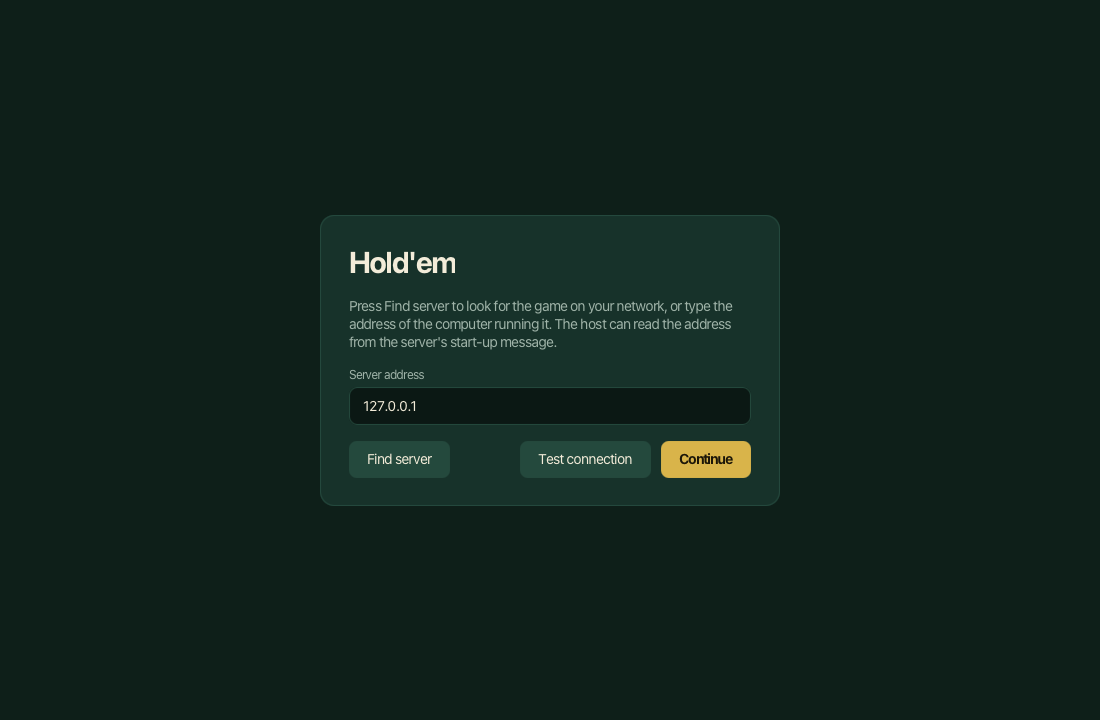
\includegraphics[width=\linewidth]{images/app-1-connect.png}
  \caption{Connecting to the server}
\end{subfigure}\hfill
\begin{subfigure}{0.49\textwidth}\centering
  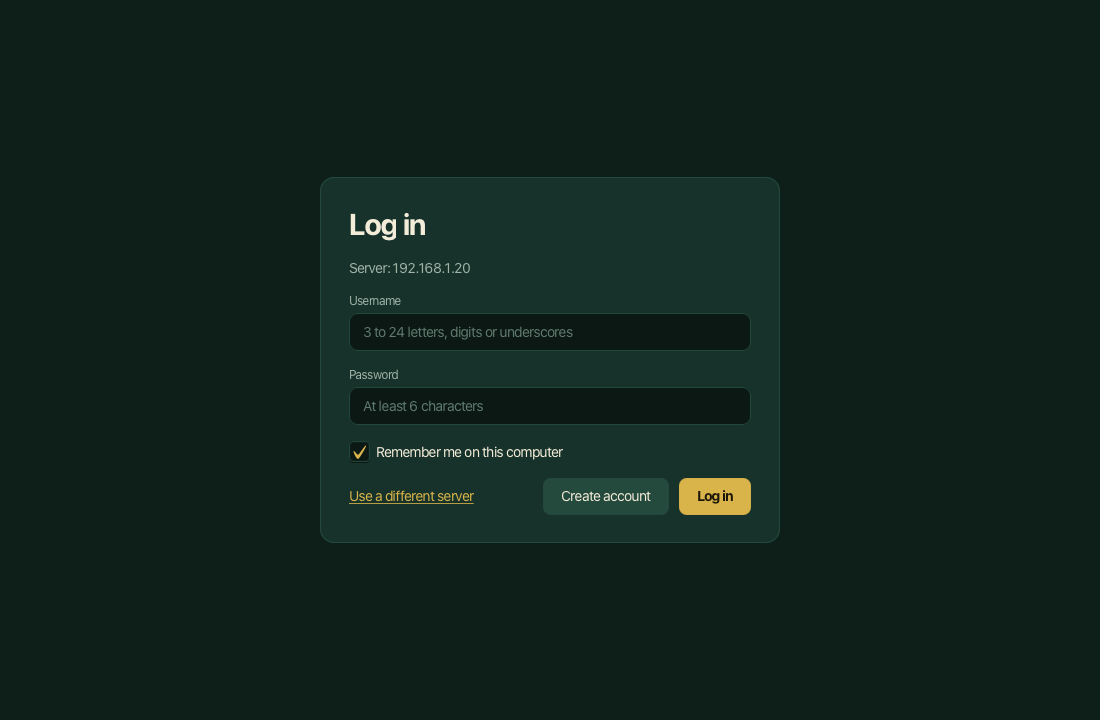
\includegraphics[width=\linewidth]{images/app-2-login.png}
  \caption{Logging in}
\end{subfigure}
\\[8pt]
\begin{subfigure}{0.49\textwidth}\centering
  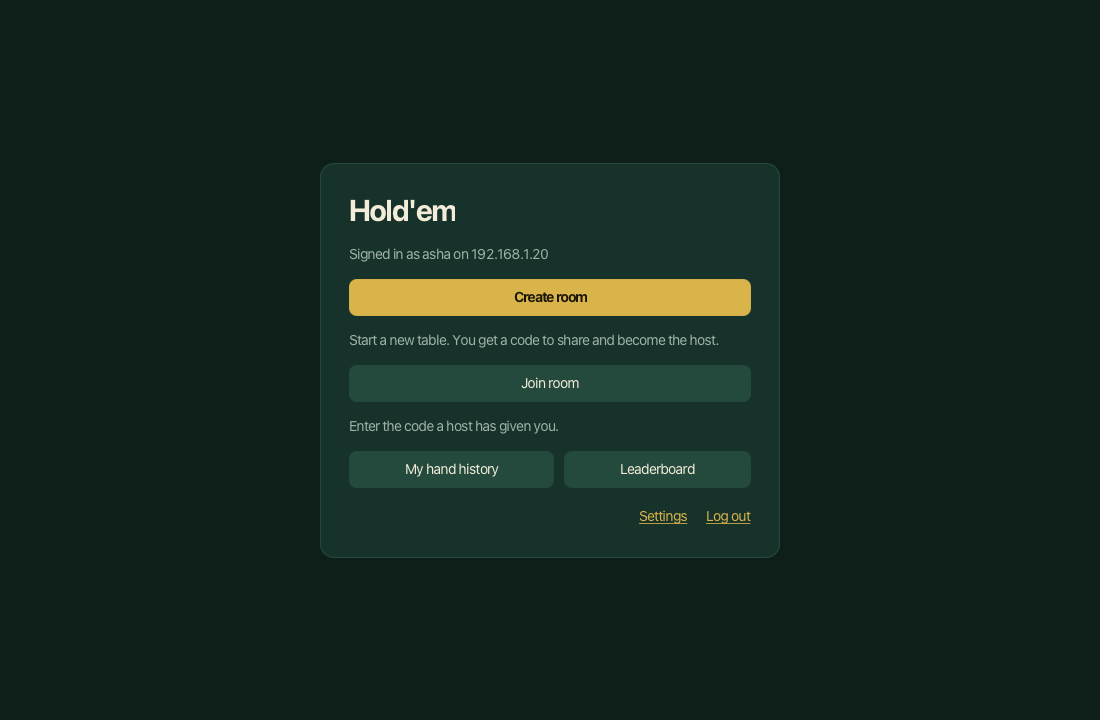
\includegraphics[width=\linewidth]{images/app-3-home.png}
  \caption{Home: create or join a room}
\end{subfigure}\hfill
\begin{subfigure}{0.49\textwidth}\centering
  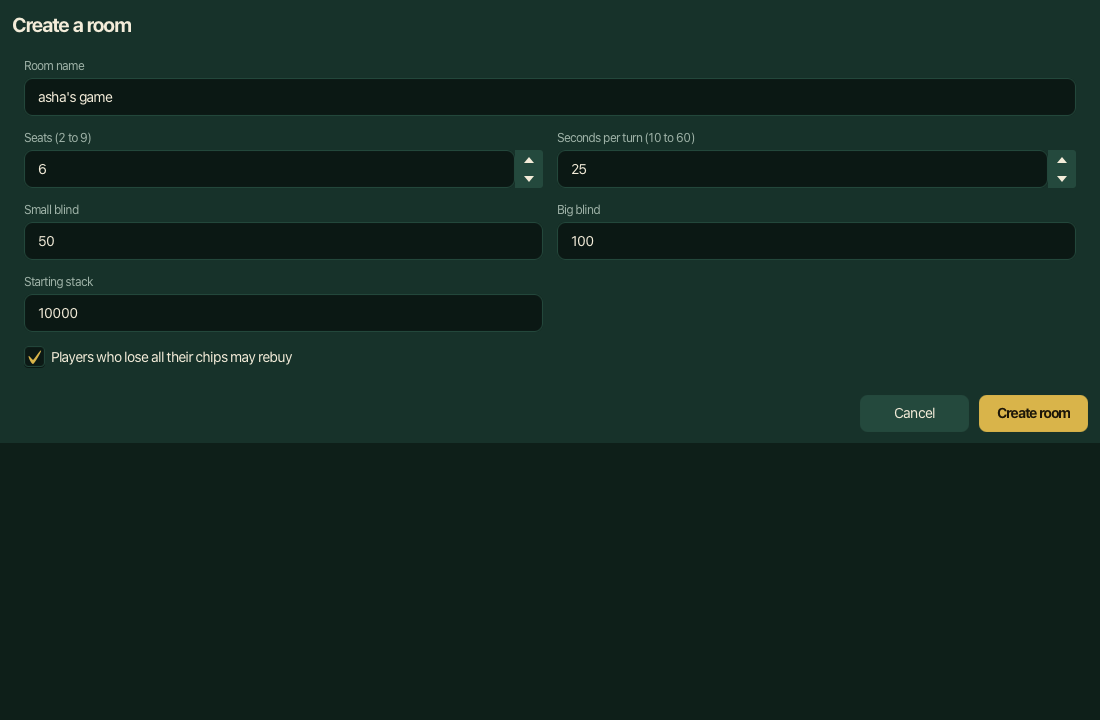
\includegraphics[width=\linewidth]{images/app-4-create-room.png}
  \caption{Room settings}
\end{subfigure}
\caption{Getting into a game.}
\end{figure}

\begin{figure}[H]
\centering
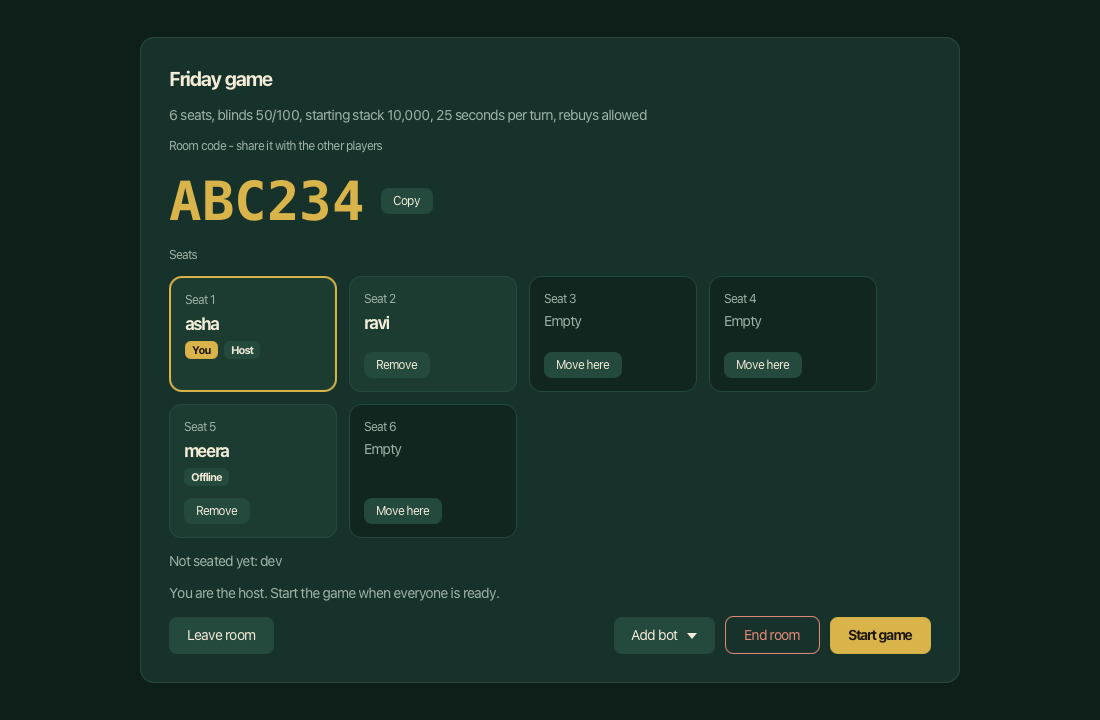
\includegraphics[width=0.85\textwidth]{images/app-6-waiting-host.png}
\caption{The waiting room seen by the host, with the room code to share, seat controls and the
\emph{Add bot} menu.}
\end{figure}

\begin{figure}[H]
\centering
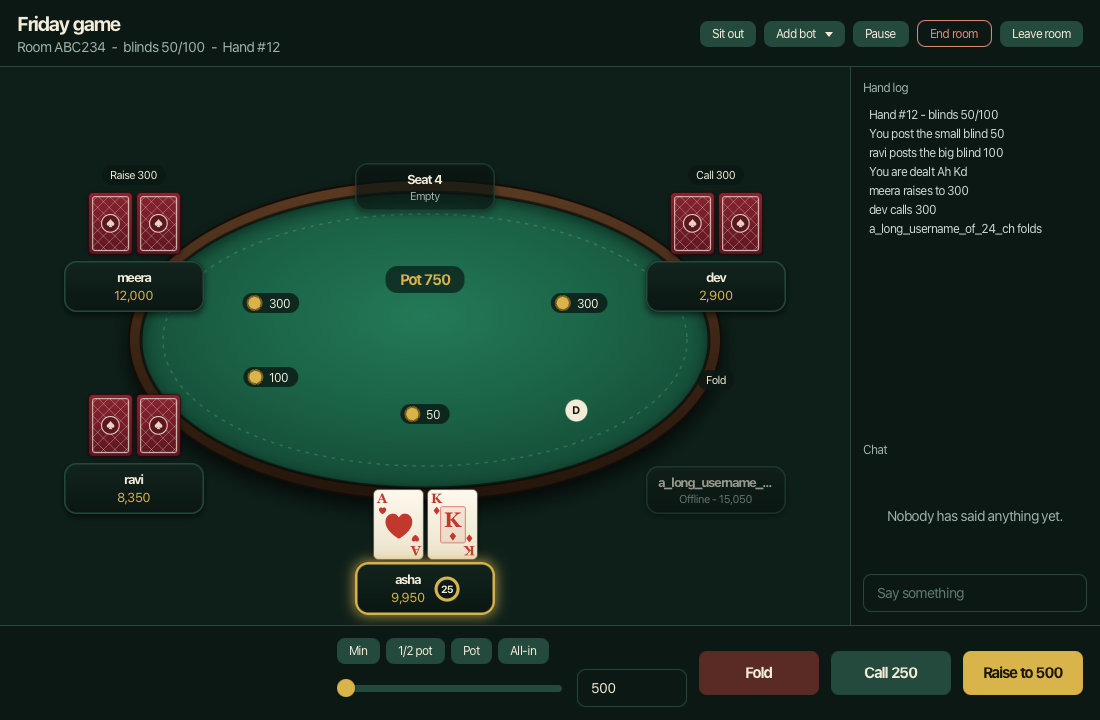
\includegraphics[width=0.85\textwidth]{images/app-7-table-your-turn.png}
\caption{At the table on the player's turn: the action buttons and bet slider at the bottom, the
hand log and chat on the right.}
\end{figure}

\begin{figure}[H]
\centering
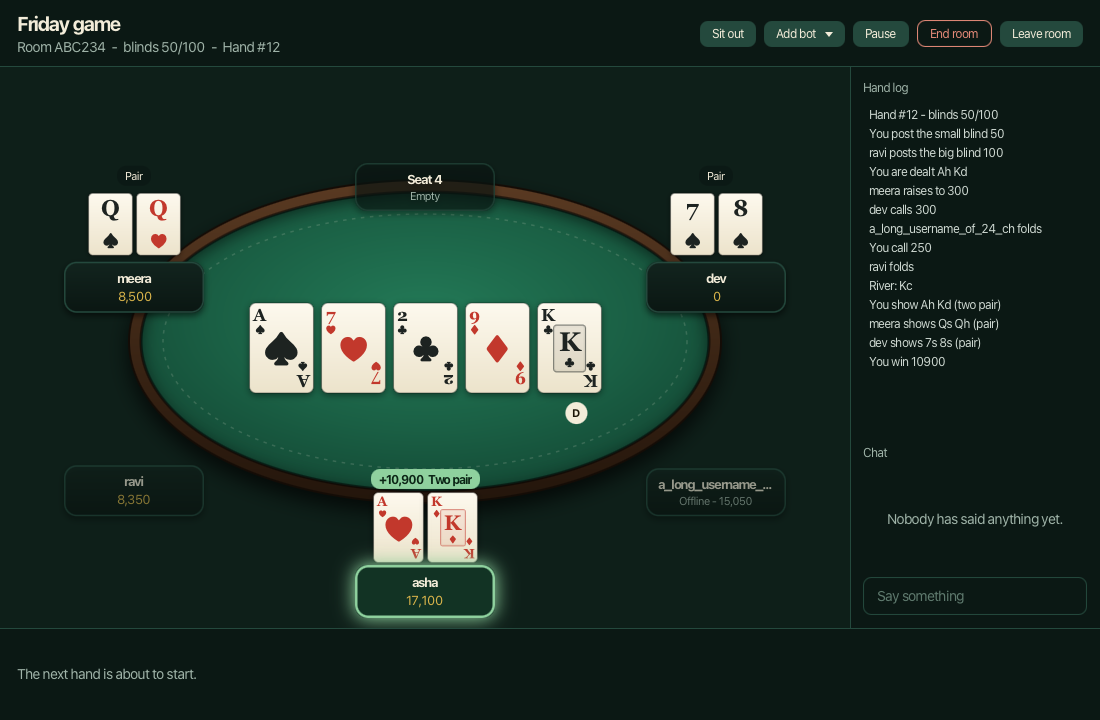
\includegraphics[width=0.85\textwidth]{images/app-7-table-showdown.png}
\caption{A showdown: the remaining players' cards are turned over and the winner is marked.}
\end{figure}

\subsection{Web pages}
Anyone on the network can open these in a browser at \cls{http://<host-ip>:8080/poker/}.

\begin{figure}[H]
\centering
\begin{subfigure}{0.49\textwidth}\centering
  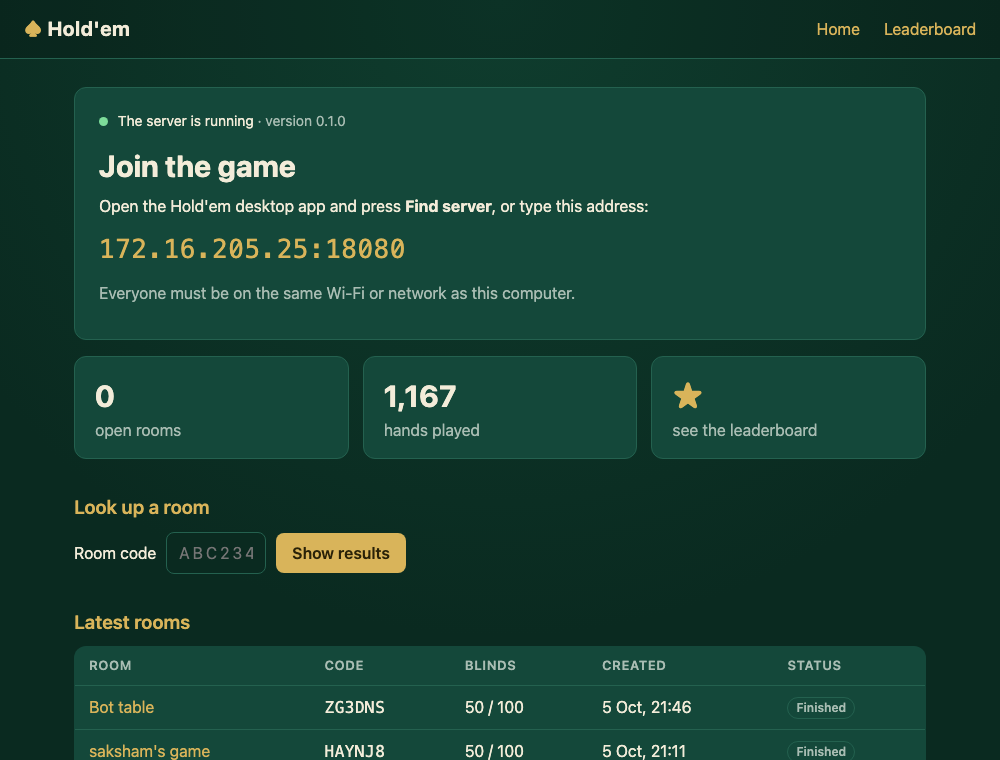
\includegraphics[width=\linewidth]{images/web-home.png}
  \caption{Home page}
\end{subfigure}\hfill
\begin{subfigure}{0.49\textwidth}\centering
  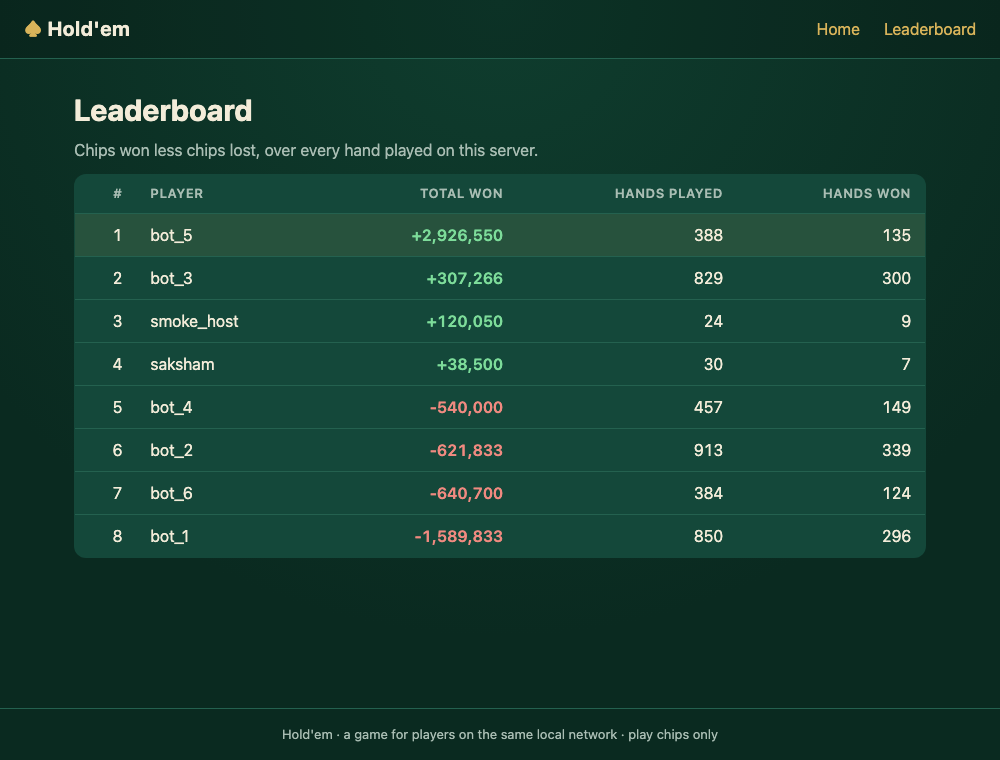
\includegraphics[width=\linewidth]{images/web-leaderboard.png}
  \caption{Leaderboard}
\end{subfigure}
\caption{JSP pages served by the server.}
\end{figure}

\begin{figure}[H]
\centering
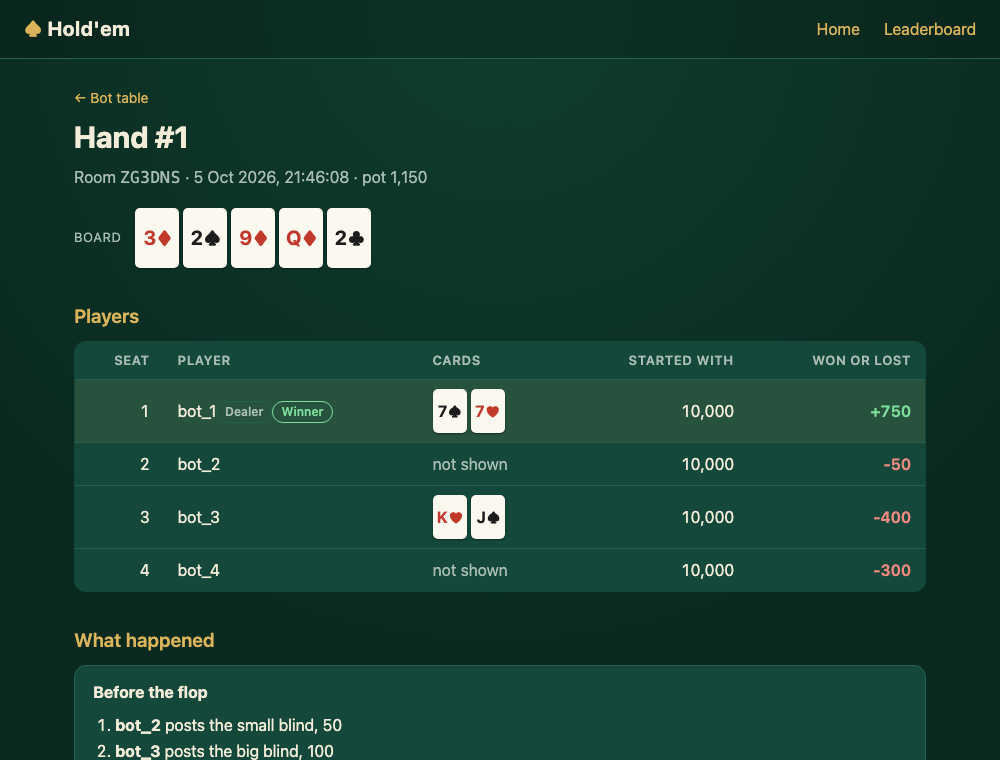
\includegraphics[width=0.75\textwidth]{images/web-replay.png}
\caption{Replay of a saved hand, action by action.}
\end{figure}

% ---------------------------------------------------------------- 8
\section{Testing}

The project has more than 470 automated JUnit tests, run with \cls{./mvnw clean verify}.
\begin{itemize}
\item \textbf{Engine:} betting rules, minimum raises, all-ins, side pots with up to nine
players, and the hand evaluator checked against every hand category. Each test hand uses a
fixed deck, and chips are checked to be conserved.
\item \textbf{Server:} rooms are driven command by command through a test harness, including
reconnecting, kicking players, rebuys and the turn timer. A separate test checks that no
message ever carries another player's hole cards.
\item \textbf{Database:} DAO tests run against a real PostgreSQL in a temporary schema.
\item \textbf{Bots:} a test seats real bots on real threads for hundreds of hands.
\item \textbf{Load:} the bot client plays hundreds of hands over the network; afterwards the
number of hands in the database must match.
\end{itemize}

% ---------------------------------------------------------------- 9
\Needspace{14\baselineskip}\section{Conclusion and future work}

Oak Hold'em is a complete, working poker game for a local network. It plays correct No-Limit
Texas Hold'em for up to nine players, keeps every player's cards private, saves every hand,
and offers computer players at three levels. Splitting it into modules kept the game rules
separate from the network, the database and the windows, which made each part easy to test on
its own. Every topic of the Java syllabus appears in a place where it does real work.

Possible next steps are a tournament mode with rising blinds, spectators who can watch a
table, and a stronger computer player built on game-theory methods.

\end{document}
